\documentclass[12pt,a4paper]{article}
\usepackage{geometry}
\newgeometry{tmargin=2cm, bmargin=2cm, lmargin=2cm, rmargin=2cm}
\usepackage[T1]{fontenc}
\usepackage[polish]{babel}
\usepackage[utf8]{inputenc}
\usepackage{amsmath}
\usepackage{amssymb}
\usepackage{graphicx} % Usunięto [dvips] dla lepszej kompatybilności
\usepackage{listings}
\usepackage[usenames,dvipsnames]{xcolor}

\definecolor{mygreen}{RGB}{25,130,0}
\definecolor{mylilas}{RGB}{180,55,230}
\definecolor{myNumbers}{RGB}{180,222,230}

\lstloadlanguages{Matlab}
\lstset{language=Matlab,
    breaklines=true,
    basicstyle=\ttfamily,
    columns=fullflexible,
    extendedchars=true,
    inputencoding=utf8,
    keepspaces=true,
    morekeywords={matlab2tikz},
    keywordstyle=\color{blue},
    identifierstyle=\color{black},
    stringstyle=\color{mylilas},
    commentstyle=\color{mygreen},
    showstringspaces=false,
    emph=[1]{if,while,for,end,break,function,return,error,disp,syms},
    emphstyle=[1]\color{red},
    tabsize=2,
    xleftmargin=2em,
    frame=single,
    framexleftmargin=1.5em,
    literate={ą}{{\k{a}}}1
           {ę}{{\k{e}}}1
           {ć}{{\'c}}1
           {ł}{{\l{}}}1
           {ń}{{\'n}}1
           {ó}{{\'o}}1
           {ś}{{\'s}}1
           {ź}{{\'z}}1
           {ż}{{\.z}}1
           {Ą}{{\k{A}}}1
           {Ę}{{\k{E}}}1
           {Ć}{{\'C}}1
           {Ł}{{\L{}}}1
           {Ń}{{\'N}}1
           {Ó}{{\'O}}1
           {Ś}{{\'S}}1
           {Ź}{{\'Z}}1
           {Ż}{{\.Z}}1,
}

\begin{document}

\section*{Zadanie 2}

Najprostszy model wykładniczy rozwoju pojedynczej populacji (model Malthusa)
otrzymuje się zakładając, że populacja ma warunki nieograniczonego rozwoju, w
tym np. że każdy osobnik ma nieograniczony dostęp do pożywienia i miejsc lęgowych. Przyjmuje się ponadto, że wszystkie osobniki są równomiernie rozlokowane
przestrzennie i jednakowe — są zdolne do partenogenezy i wydają na świat regularnie tyle samo potomków. W takim abstrakcyjnym przypadku średnią liczebność
populacji $N(t)$ (w chwili $t$) można obliczyć z zależności

\begin{equation*}
    N'(t) = rN(t),
\end{equation*}
gdzie $r$ oznacza współczynnik rozrodczości netto dla populacji $N$ (różnica między
współczynnikiem rozrodczości a śmiertelności). Przeanalizować za pomocą funkcji
\texttt{ode45} powyższe równanie dla $N(0) = 100$ i

\begin{itemize}
    \item[(a)] $r > 0$;
    \item[(b)] $r = 0$;
    \item[(c)] $r < 0$.
\end{itemize}
Jak można zinterpretować zachowanie się populacji pod względem biologicznym w
każdym z powyższych przypadków? \textbf{Porównać} otrzymane wyniki z rozwiązaniem
otrzymanym analitycznie lub symbolicznie (\texttt{dsolve}). Zamieścić otrzymane wykresy.

\vspace{1em}

\begin{lstlisting}
t_span = [0 5];
N_0 = 100;

r_a = 0.5;
ode_a = @(t, N) r_a * N;
[T_a ,N_a] = ode45(ode_a,t_span,N_0);

r_b = 0;
ode_b = @(t, N) r_b * N;
[T_b, N_b] = ode45(ode_b,t_span,N_0);

r_c = -0.5;
ode_b = @(t, N) r_c * N;
[T_c, N_c] = ode45(ode_b,t_span,N_0);

figure;
hold on;
plot(T_a, N_a, 'g');
plot(T_b, N_b, 'b');
plot(T_c, N_c, 'r');
xlabel('Czas t');
ylabel('Liczebność populacji N(t)');
legend('r>0','r=0','r<0',Location='best')
title('Model Malthusa (ode45)')
grid on;
axis tight;
hold off;
\end{lstlisting}

\begin{figure}[h]
    \centering
    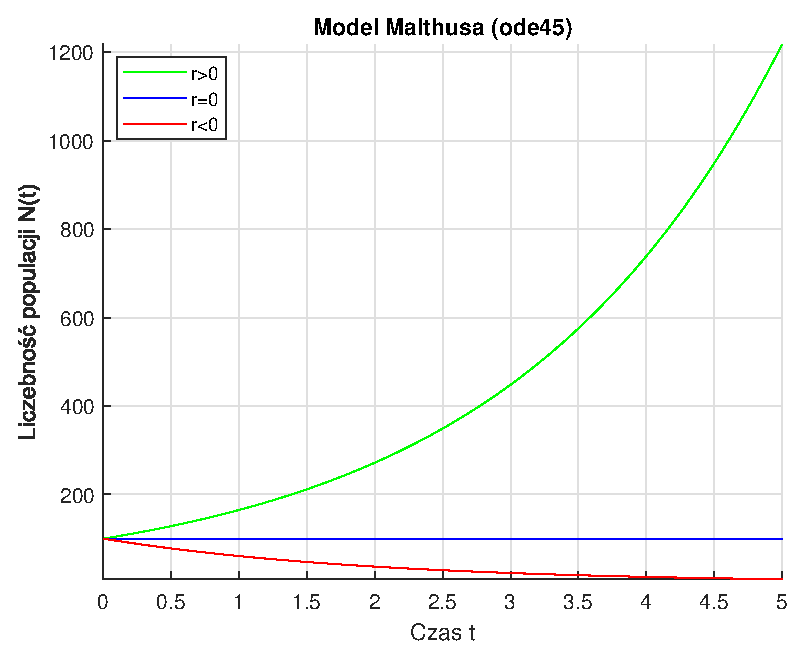
\includegraphics[width=0.8\textwidth]{wykres_malthusa.eps}
    \caption{Wykres przedstawiający Model Malthusa dla różnych współczynników r.}
    \label{fig:wykresy}
\end{figure}

\vspace{2em}

Jak można zinterpretować zachowanie się populacji pod względem biologicznym?

\begin{itemize}
    \item Przypadek $r > 0$ (zielona krzywa)
    Współczynnik urodzeń jest wyższy niż współczynnik zgonów. Prowadzi to do eksplozji demograficznej.
    \item Przypadek $r = 0$ (niebieska krzywa)
    Stan równowagi idealnej. Liczba narodzin dokładnie równoważy liczbę zgonów. Środowisko jest stabilne, a populacja ani się nie rozwija, ani nie kurczy
    \item Przypadek $r < 0$ (czerwona krzywa)
    Populacja wymiera. Śmiertelność przewyższa rozrodczość. Matematycznie dąży do zera, biologicznie gatunek przestaje istnieć, gdy liczebność spadnie poniżej 1.
\end{itemize}

\newpage

\begin{lstlisting}
syms N(t) r
tspan = [0 5];

eqn = diff(N, t) == r * N;

n_symbolicznie = dsolve(eqn, N(0) == 100);

pretty(n_symbolicznie);

r_test_a = 0.5;
[T_num_a, N_num_a] = ode45(@(t,N) r_test_a*N, tspan, 100);
wzor_a = subs(n_symbolicznie, r, r_test_a);

r_test_b = 0;
[T_num_b, N_num_b] = ode45(@(t,N) r_test_b*N, tspan, 100);
wzor_b = subs(n_symbolicznie,r, r_test_b);

r_test_c = -0.5;
[T_num_c, N_num_c] = ode45(@(t,N) r_test_c*N, tspan, 100);
wzor_c = subs(n_symbolicznie,r, r_test_c);

figure;
hold on;
fplot(wzor_a, tspan, 'g-'); 
fplot(wzor_b, tspan, 'b-'); 
fplot(wzor_c, tspan, 'r-'); 
plot(T_num_a, N_num_a, 'ro');
plot(T_num_b, N_num_b, 'go');
plot(T_num_c, N_num_c, 'bo');
title('Porównanie: Numeryczne (kółka) vs Symboliczne (linie)');
xlabel('Czas t');
ylabel('Liczebność populacji N(t)');
grid on;

print -depsc wykres_porównanie.eps
\end{lstlisting}

\newpage

Uruchomienie części kodu z \texttt{dsolve} zwróci wynik: 
\vspace{1em}
\begin{lstlisting}
    100 exp(r t)
\end{lstlisting}
\vspace{1em}
Jest to dokładny opis matematyczny krzywych, które dostaliśmy numerycznie:
\begin{itemize}
    \item Gdy $r > 0$ , funkcja wykładnicza rośnie ($100e^{0.5t}$).
    \item Gdy $r=0, e^0 = 1$, więc $N(t) = 100 \cdot 1 = 100$ (stała).
    \item Gdy $ r< 0 $, funkcja wykładnicza maleje ($100e^-{0.5t}$).
\end{itemize}
Wnioski z zadania są kompletne: metoda numeryczna \texttt{ode45} w MATLABie daje wyniki idealnie zgodnie z teorią matematyczną (rozwiązaniem analitycznym).

\vspace{1em}

\begin{figure}[h]
    \centering
    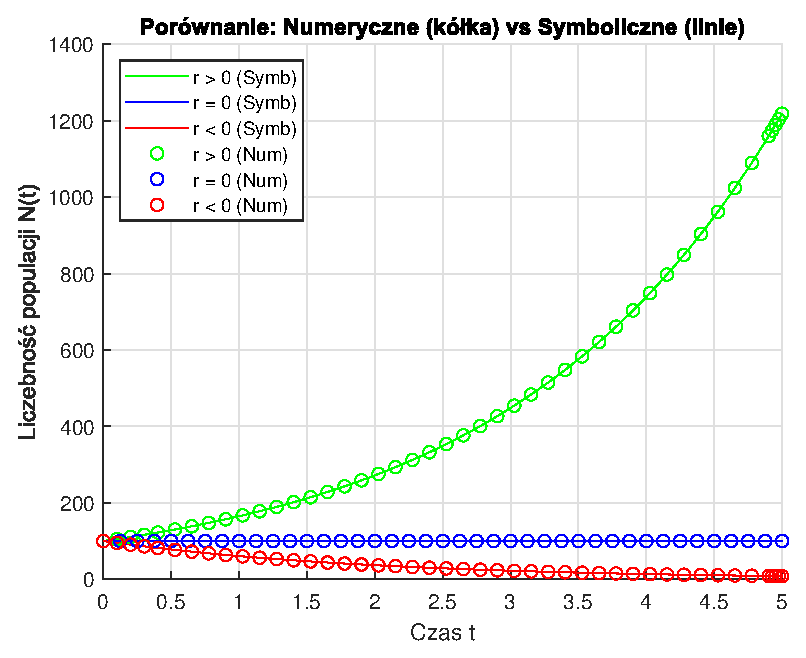
\includegraphics[width=0.8\textwidth]{wykres_porównanie.eps}
    \caption{Wykres przedstawiający porównanie rozwiązań numerycznych i symbolicznych modelu Malthusa w określonych warunkach}
    \label{fig:wykresy}
\end{figure}

\end{document}